\chapter{Unsupervised Learning of Cross-lingual Word Embedding}
Chapter 3 introduces the supervised learning of cross-lingual word embedding, they employ parallel data like bilingual dictionary or parallel corpora and have shown strong results on a word retrieval task.  However, labeling the lexicon information still costs lots of labor. This motivates people to explore fully unsupervised method. In this chapter, several unsupervised approaches will be explained including a novel corpus-based approach, which is distinct from other methods by exploiting an extra language model and corpus-based training process. All these approaches contains an iterative training procedure. 
\section{Initialization}
Pre-trained monolingual embeddings capture distribution information for each language. These embeddings are typically not expected to be aligned between languages A good initialization is a key to the iterative training framework.
A practical approach for reducing the need of bilingual supervision is to design heuristics to build the seed dictionary. \cite{hauer2017bootstrapping} propose to use shared words and cognates to extract the seed dictionary. This method has a flaw that it depends on the writing system. \cite{artetxe2018robust} raise a method that using similarity matrix to capture rough cross-lingual signals.\\

\subsection{Heuristics}
The seed is constructed by identifying words with similar spelling (cognates). A relative-frequency constraint is imposed to filter out word pairs that have fully different meaning; generate the list of words by frequency first, for each source word, if there exists target word that the normalized edit distance (NED) and absolute difference between the respective frequency ranks is within a specific threshold, these two word will be added into a seed dictionary.  This noisy seed lexicon will be considered as initial signals. There is no one-to-one constraint, so both source and target words may appear multiple times in the seed. 

\subsection{Similarity Matrix}
Similarity matrix is based on a simple assumption: while the axes of the original ${\lvert \tilde{V} \rvert}$ most frequent embeddings ${F \in \mathbb{R}^{d \times {\lvert \tilde{V} \rvert} }}$ and ${E \in \mathbb{R}^{d \times {\lvert \tilde{V} \rvert} }}$  are different, but $M_F=F^{\top}F$, $M_E = E^{\top}E$ capture the similarity inner respective languages. The similarity matrices $M_F$ and $M_E$ would be equivalent up to a permutation of their rows and columns. For example, in one language, the similarity between $a,b,c$ and $i,j,k$ is as the left graph in Figure 4.1, suppose ideal the their corresponding translations are $a^{\prime},b{\prime},c{\prime}$ and $i{\prime},j{\prime},k{\prime}$, but the order differs as the middle graph. If we first sort the values in each row, it will be much easier to find the relationship between $a$ and $a^{\prime}$, etc.. They find $\sqrt{M_F}$ and $\sqrt{M_E}$ 
work better in practice.
\begin{figure}[H]
	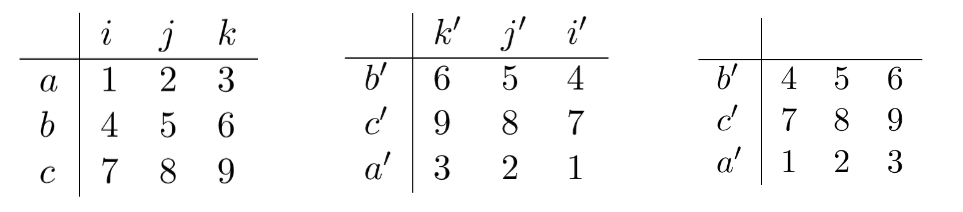
\includegraphics[width=12cm]{similarity}
	\centering
	\caption{Illustration of similarity matrix method}
\end{figure}

While the latter is far from the accurate alignment, it works well as the initialization for the iterative methods described next.
\section{Vocabulary-based Learning}
The vocabulary-based approach depends on high-quality lexical information to learn the mapping between embedding distributions.
We can use Figure 4.2 to illustrate the vocabulary-based learning process. As in graph (A) there are two distributions of word embeddings, source words in red denoted by $F$ and target words in bleu denoted by $E$, which we want to align. Each dot represents a word in shared space. Using initialization, we learn a rotate matrix $W$ which roughly aligns the two distributions. According to dictionary induction, we can find some reliable points in graph (B). We can futher refine the mapping $W$, using frequent words aligned by the previous step as anchor points, and minimizes a loss function measured by mapping distance as in graph (C). Repeat steps in (B) and (C), we hope to find a liner mapping that can be generalized to all words in the dictionary as in graph (D).
\begin{figure}[H]
	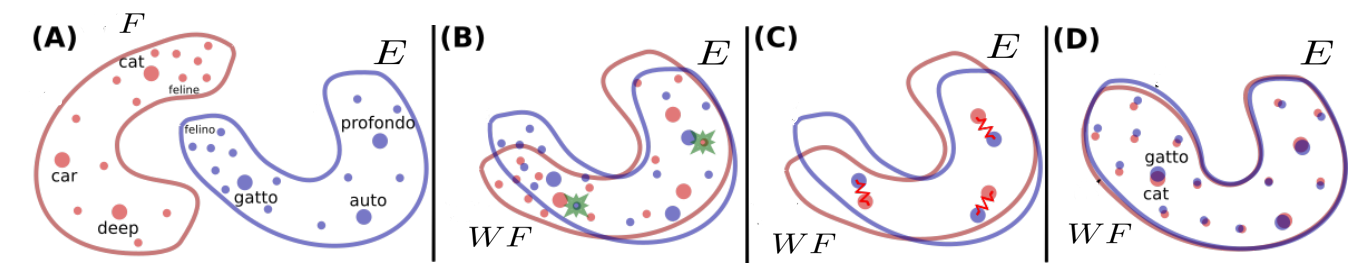
\includegraphics[width=12cm]{vocab}
	\centering
	\caption{Illustration of vocabulary-based learning (\cite{conneau2017word})}
\end{figure}
\subsection{Iterative Procrustes Analysis}
After initialization, the words in the seed dictionary can be considered as temporary  anchor points for Procrustes analysis, which has been introduced in Section 3.2.1.
Apply the Procrustes solution on the current seed dictionary, use the learned mapping matrix $W$ and dictionary induction technique to construct a better seed dictionary again. Repeat such process we suppose to obtain a hopefully better mapping and dictionary until some convergence criterion is met. The training will be stopped when the improvement on the average dot product for the induced dictionary falls below a give threshold from one iteration to the next. In practice, the threshold value is set at $1e-6$.  To prevent the mapping and dictionary from getting stuck in local optima, Mutual nearest neighbors and thresholding are used to ensure a high-quality dictionary. In the experiments we find that intersection of two unidirectional dictionaries work better than union or a unidirectional dictionary,  that is to say, the quality of dictionary plays more important role than the quantity.\\
\begin{figure}[h]
	\centering
	\begin{minipage}{.7\linewidth}
		\begin{algorithm}[H]
			\SetAlgoLined
			\KwIn{$F$ (source embeddings)}
			\KwIn{$E$ (target embeddings)}
			\KwIn{$dico$ (seed dictionary)}
			\KwResult{$W$ (embedding mapping) }
			\While{not converge}{
				${W \leftarrow LEARN\_MAPPING(F,E,dico)}$
				${dico \leftarrow LEARN\_DICTIONARY(W)}$
				
			}
			\caption{Iterative training procedure}
		\end{algorithm}
	\end{minipage}
\end{figure}

\subsection{Adversarial Training (GANs)}
The adversarial training was for cross-lingual embedding mapping is first proposed by \cite{barone2016towards}, who combines an encoder that maps source word embeddings into the target embedding space, a decoder that reconstructs the source embeddings from the mapped embeddings and a discriminator that discriminates between embeddings. \cite{zhang2017adversarial} incorporate additional techniques like noise injections to aid the training. \cite{conneau2017word} finally achieve good results by dropping the reconstruction component regularizing the mapping to be orthogonal\\
Let ${=\{ \bm{f}_1, \cdots, \bm{f}_{{\lvert \tilde{V} \rvert}}\}}$ and ${ = \{ \bm{e}_1, \cdots , \bm{e}_{{\lvert \tilde{V} \rvert}}\}}$ be the most ${\lvert \tilde{V} \rvert}$ frequent word embeddings from source and target languages respectively. We refer the discriminator parameters as ${\theta_D}$.The discriminator is a multi-layer neural network trained to discriminate the transformed source word embedding from the target word embedding, while the mapping $W$, as simple as a linear transformation, is trained to fooling discriminator. In the two-player game, mapping from source embedding space to the target space is supposed to be learned.\\

Generator loss 
\[ \mathcal{L_G}(W|\theta_D) =  -\frac{1}{{\lvert \tilde{V} \rvert}} \sum_{n=1}^{\tilde{V}}\log P_{\theta_D}(source=0|W \bm{f}_n) - \frac{1}{\tilde{V}} \sum_{n=1}^{{\lvert \tilde{V} \rvert}} \log P_{\theta_D}(source = 1 | \bm{e}_n) \]
Discriminator loss
\[ \mathcal{L_D}(\theta_D | W) =  -\frac{1}{{\lvert \tilde{V} \rvert}} \sum_{n=1}^{{\lvert \tilde{V} \rvert}} \log P_{\theta_D}(source = 1| W\bm{f}_n) - \frac{1}{{\lvert \tilde{V} \rvert}} \sum_{n=1}^{{\lvert \tilde{V} \rvert}} \log P_{\theta_D}(source=0| \bm{e}_n) \]	 
\section{Corpus-based Learning}
\subsection{Motivation}
The vocabulary-based training approach makes good use of the  embedding distribution similarity. However, it just looks at the mutual nearest neighbors, not considering polysemy of the words.  It does not take the semantic or contextual information into consideration when training the cross-lingual mapping, which would be a flaw especially in machine translation task. We also argue that word frequency should also be considered when training. For example, though words are synonyms, some of them are more used than others. When inducing the lexicon, we should assign priority to frequent words.\\
In if we translate corpus, we can consider those various translations to make the mapping better 
The intuition of corpus-based approach is that, if we integrate the translation task into the cross-lingual mapping learning process, the factors mentioned above will be taken into account; with information provided from LM, different translation candidates will be chosen. Also  LM prefers the common words. 
\subsection{Framework}
 We propose a novel corpus-based learning approach by integrating corpus translation task. We build a word-based machine translation, in this thesis simplified as a word-by-word translation system, which exploits dictionary induction as lexical model. The intuition is that if the translation system gets improved better translation, we can further learn a better mapping based on the word translation pairs. LM is used to improve the translation. In the closed-loop learning process by alternating corpus translation and embedding mapping learning, we are hopefully learn good mapping matrix at last. Algorithm 3 summarize such iterative framework I propose. We use neural network with only one layer to represent the mapping matrix $W$, train successively with stochastic gradient updates to minimize the distance measurement.\\
\begin{figure}[H]
	\centering
	\begin{minipage}{.7\linewidth}
		\begin{algorithm}[H]
			\SetAlgoLined
			\KwIn{$F$ (source embeddings)}
			\KwIn{$E$ (target embeddings)}
			\KwIn{$\textbf{LM}_e$ (language model)}
			\KwIn{$\mathcal{F}$ (source corpus)}
			\KwResult{$W$ (embedding mapping)}
			\While{not converge}{
				${\ \  \mathcal{E} \leftarrow TRANSLATE(\mathcal{F}, F, E, \textbf{LM}_e)}$ 
				${W \leftarrow LEARN\_MAPPING(\mathcal{F}, \mathcal{E})}$				
			}		
			\caption{Iterative learning of corpus-based approach}
		\end{algorithm}
	\end{minipage}
\end{figure}

%We propose to use the output word-by-word translation as the input of the mapping learning system. Assuming that the quality of word-by-word translation was indeed better than the previous one. The mapping learning system should be able to learn a better mapping and, consequently, an ever better translation the second time. The process can then be repeated iteratively to obtain a hopefully better maping and translation each time until some convergence point was met. 

This corpus-based approach combines mapping learning, dictionary induction and corpus translation. The efficiency turns out to be critical. Actually, the learning time depends mainly on the corpus size. It will be very costly if we translate the entire source corpus especially at the beginning stage, when the improvement of the mapping is relative slow and more training iterations are required. In order to solve this, I propose an online learning method, which can greatly improve the training efficiency. 

\subsection{Online Training}

\begin{figure}[H]
	\centering
	\begin{minipage}{.7\linewidth}
		\begin{algorithm}[H]
			\SetAlgoLined
			\KwIn{$F$ (source embeddings)}
			\KwIn{$E$ (target embeddings)}
			\KwIn{$\textbf{LM}_e$ (language model)}
			\KwIn{$\mathcal{F}$ (source corpus)}
			\KwResult{$W$ (embedding mapping) }
			\While{not converge}{
				\ \ Generate batch of source sentences $\{f_1^J\}$ from $\mathcal{F}$\\
				${\{e_1^I\} \leftarrow TRANSLATE(\{f_1^J\}, F, E, \textbf{LM}_e) }$ 
				${W \leftarrow LEARN\_MAPPING(\{f_1^J\}, \{e_1^I\})}$				
			}		
			\caption{Online learning for corpus-based approach}
		\end{algorithm}
	\end{minipage}
\end{figure}
Instead of translate the entire corpus, each time I iterate over the corpus to generate specific number of sentences as a sentence batch. After translation is done, we extract the word translation pairs as seed dictionary. For more complicated word-based machine translation system, extraction will requires the alignment information. In my word-by-word translation system, I just use the word translation pairs at each position. We could improve the quality of seed dictionary by filtering the pairs, which could be noise in the dictionary according to statistical information. We train the mapping using neural network trained with SGD. Mapping learned on current sentence batch is used to induce the lexicon for translation of next sentence batch. The efficiency of this online algorithm mainly depends on the corpus size and batch size. We can either extend the corpus size or train over the same corpus more than once since this approach is data-driven method.


\subsection{Training Details}
\begin{itemize}
	
\item Embedding Normalization\\
We start with a pre-processing that normalize the embeddings, mean the centers of each dimension and then normalize again. We take three steps in order to obtain normalized embeddings with unit length and centering near zero. As in both CBOW and skip-gram model, the prediction probability is calculated with the inner product of embeddings. By normalization, the inner product falls back to the cosine distance, and cosine distance the criterion we used for nearest neighbors search. In addition to this, the orthogonal constraint preserves the length normalization and cosine similarity after the projection. Hence normalization helps to keep the consistence between embedding learning and dictionary induction (\cite{xing2015normalized}). After normalization, all embeddings are located on a hypersphere. Dimension-wise mean centering ensures that the expected inner product of two random embeddings  consequently, the cosine similarity, is zero (\cite{artetxe2016learning}).
%These steps are shown to be beneficial (\cite{artetxe2016learning}).

	\item Dictionary Induction
	\begin{itemize}
		\item CSLS retrieval
		 With cross-lingual word embeddings, we can directly find the word translation using nearest neighbors search. The nearest neighbor suffers from the hubness problem. As mentioned in Section 3.4, we adopt the Cross-domain Similarity Local Scaling (CSLS) from \cite{conneau2017word}. Following the authors, we set $k=10$.
		 \item Frequency-based vocabulary cutoff\\
		 The complexity for dictionary induction grows with respect to target vocabulary size. This increases not only  computation cost, but also the number of possible translations. In the experiments we find out that those less frequent words can be noise since less words are less trained. These noise word translations would have global negative influence of the sentence translation.
		 We propose to restrict the vocabulary size to the k-top frequent words in the source and target languages, where we find $k=50000$ can balance the efficiency and accuracy.	 
	\end{itemize}


	\item Corpus Translation\\
	Most words have multiple translations, some are more likely than others. Also the translation depends on the context. For example, 'home', 'house' are synonyms, but when translating 'zu Haus', we will choose 'home'. By integrating LM, we can choose better word translation as well as sentence translation according to contextual information. We exploit a $5$-gram LM trained by KenLM (\cite{heafield2011kenlm}) and use a linear mapping to convert the cosine similarity to lexical probability. I improve the translation efficiency greatly by implementing a context-aware beam search with beam size 10. 
		\[ \hat{e}_1^J = \argmax{e_1^J}{\ \prod_{i=1}^{J}} {P^{\lambda_{LM}}(e_i|e_{i-4}^{i-1}) \cdot Q^{\lambda_{lex}}(f_i,e_i)}\]
		where $P(\cdot)$ and $Q(\cdot)$ are scores predicted respectively by LM and cross-lingual word embeddings. Both scores are in range $[0,1]$. 
	More details will be explained in Chapter 5.
	



	
	\item Optimization Objective \\
	Suppose we have got translation, we can extract word translation pairs as seed dictionary $dico$. The goal of optimization is to find the best mapping so that the mapping is more general to cover as much as possible lexicon with high accuracy. In this theis, linear mapping $W \in \mathbb{R}^{d \times d}$ will be trained to minimize a self-defined loss function between mapped  source word embeddings target word embeddings.
	\[ W = \argmin{W \in \mathbb{R}^{d \times d}} \frac{1}{{\lvert \tilde{V} \rvert}} \sum_{n=1}^{\lvert \tilde{V} \rvert} l(W\bm{f}_n, \bm{e}_n) \]
	where $l$ is a loss function, in this thesis I compare the results of Euclidean distance loss and cosine similarity loss and find the difference is small.\\
	To train our model, we follow the standard training procedure of neural network. For every input sample, we minimize the loss function with stochastic gradient decent (SGD) method. Better optimizer could be used to prevent from getting stuck into local optima.
	\item Orthogonal Constraint\\
	As mentioned previously, the orthogonal preserves the quality of monolingual embeddings also dot product of vectors and  $l_2$ distance. In our experiments, we find the orthogonal constraint make training procedure converge successfully. In this thesis, the orthogonal constraint is added during the training process; we use projected gradient descent to train the neural network by alternating the training and the orthogonal constraining:
\[ W \leftarrow (1+\beta) W - \beta(WW^\top)W\] 
	where $\beta$ = 0.01  is usually found to perform well.  This method ensures that the matrix stays close to the manifold of orthogonal matrices after each update. 	
	\item Learning Rate Scheduling\\
	Two different learning rate schedulers are used in this thesis. Once we get the batch sentence translation, we can either train the mapping with the learning rate inherited from last training, or train always with the initial learning rate and keep training and updating learning rate until the learning rate drops to a minimal learning rate we predefined. The first training scheduler fits the normal online algorithm principle best but in practice we find the second scheduler trains the cross-lingual embedding more efficiently.
	\item Stop Criterion\\
	Once the results of this approach have converged to a good point, we can break the training loop early. We have considered  different factors such as the loss in the embedding training process or statistics on the translation. In practice, we find the model selection methods provided by \cite{conneau2017word} more suitable in our case. They use CSLS retrieval to generate the translations of 10k most frequent source words. And then compute the average cosine similarity between these deemed translations and use this average as validation metric. Empirically, they find that this simple criterion is better correlated with the performance on the evaluation tasks than those distance based criterion.
\end{itemize}
%Our method can be combined with word-based machine translation. This approach can be further improved  with more word-based machine translation model. We can also refine the 